%% This is an example using the illcdiss.cls.
%%
%% Author: Marco Vervoort
%%
%% Version: July 18, 2001.
%%
%%
%%
%%
\documentclass{illcdiss}

%If you use Latex2.09 instead of Latex2e, comment the \documentclass line
%and uncomment one of the following lines (depending on whether you
%also want to use MakeIndex)

%\documentstyle[12pt,epsf]{illc_diss}
%\documentstyle[12pt,makeidx,epsf]{illc_diss}

%If you want to use MakeIndex, uncomment these lines
%\usepackage{makeidx}     % only with Latex2e
%\makeindex
\usepackage[utf8]{inputenc}
\usepackage{pdfpages}

\typeout{ILLC Dissertation Example File `guide.tex' <July 21, 2001>.}

\begin{document}
\pagestyle{plain}
\pagenumbering{roman}

%%  \include the `front matter'

%% This is the standard `front matter' to be used with the illcdiss.cls
%% Latex2e document class
%%
%% Author: Maarten de Rijke
%% Current maintainer: Marco Vervoort
%%
%% Version: July, 2001
%%
%%
%% Amendment August, 2020 by Gianluca Grilletti: the nationality of the candidate should not be indicated in the titelblad, independently from the birth country
%%
%%
%%
%% MAKE SURE THAT THE FILE HAS BEEN PERSONALIZED BEFORE YOU
%% PRINT AND SHIP THE FINAL VERSION.  YOU CAN FIND ITEMS THAT NEED
%% TO BE PERSONALIZED BY SEARCHING FOR THE STRING ``%PERSONALIZE''
%%
%%
%%first of all the cover.
{\pagestyle{empty}
\newcommand{\printtitle}{%
{\Huge\bfseries The ILLC Dissertation\\[0.8cm] Style}}    %PERSONALIZE

\begin{titlepage}
\par\vskip 2cm
\begin{center}
\printtitle
\vfill
{\LARGE\bfseries John B. Goode}                           %PERSONALIZE
\vskip 2cm
\end{center}
\end{titlepage}
%
% Skip a page to start on a right page again.
% If you're printing single-sided, simply delete    %PERSONALIZE
% the following line.
%
\mbox{}\newpage
\setcounter{page}{1}

%%the very first page: the `franse pagina'
\par\vskip 2cm
\begin{center}
\printtitle
\end{center}

%%the second page: the `illc pagina'
\clearpage
\par\vskip 2cm
\begin{center}
ILLC Dissertation Series DS-200X-NN                 %PERSONALIZE
\par\vspace {2cm}
\illclogo{10cm}
\par\vspace {2cm}
\noindent%
For further information about ILLC-publications, please contact\\[2ex]
Institute for Logic, Language and Computation\\
Universiteit van Amsterdam\\
Science Park 107\\
1098 XG Amsterdam\\
phone: +31-20-525 6051\\
e-mail: {\tt illc@uva.nl}\\
homepage: {\tt http://www.illc.uva.nl/}
\end{center}
\vfill

% If you're supported by NWO adapt the following 6 lines;
% otherwise simply delete them.
%
\noindent%
The investigations were supported by the            %PERSONALIZE
Philosophy Research Foundation\linebreak (SWON), 
which is subsidized by the Netherlands 
Organization for Scientific\linebreak Research (NWO).
\par\vspace {2cm}

% If you want to add CIP data (a summary of all the data used in
% library catalogs in a standard format), uncomment the following
% three lines and add the CIP data in between
%
%\noindent%
%{\tt CIP gegevens}                                 % PERSONALIZE
%\\[4ex]                                            %PERSONALIZE

%Copyright and accreditation stuff, plus ISBN
%
\noindent%
% Copyright: put your name here
Copyright \copyright\ 200X by John B.\ Goode\\[2ex] %PERSONALIZE
% Cover design, if your cover was designed by someone else
Cover design by Bert Jones.\\                       %PERSONALIZE
%Maybe some additional info on the production of the dissertation.
%Don't forget your printing shop
Printed and bound by your printer.\\[2ex]           %PERSONALIZE
%ISBN number: ask your printing shop to obtain one for you
ISBN: 90--XXXX--XXX--X                              %PERSONALIZE

% Dedication, table of contents and acknowledgements
% are handled in the main file


%%the third and fourth page, the `titelblad' and promotores-list, will be sent to you by the Pedel. Replace the file 'titlepage_from_pedel.pdf' by what you receive.
\clearpage
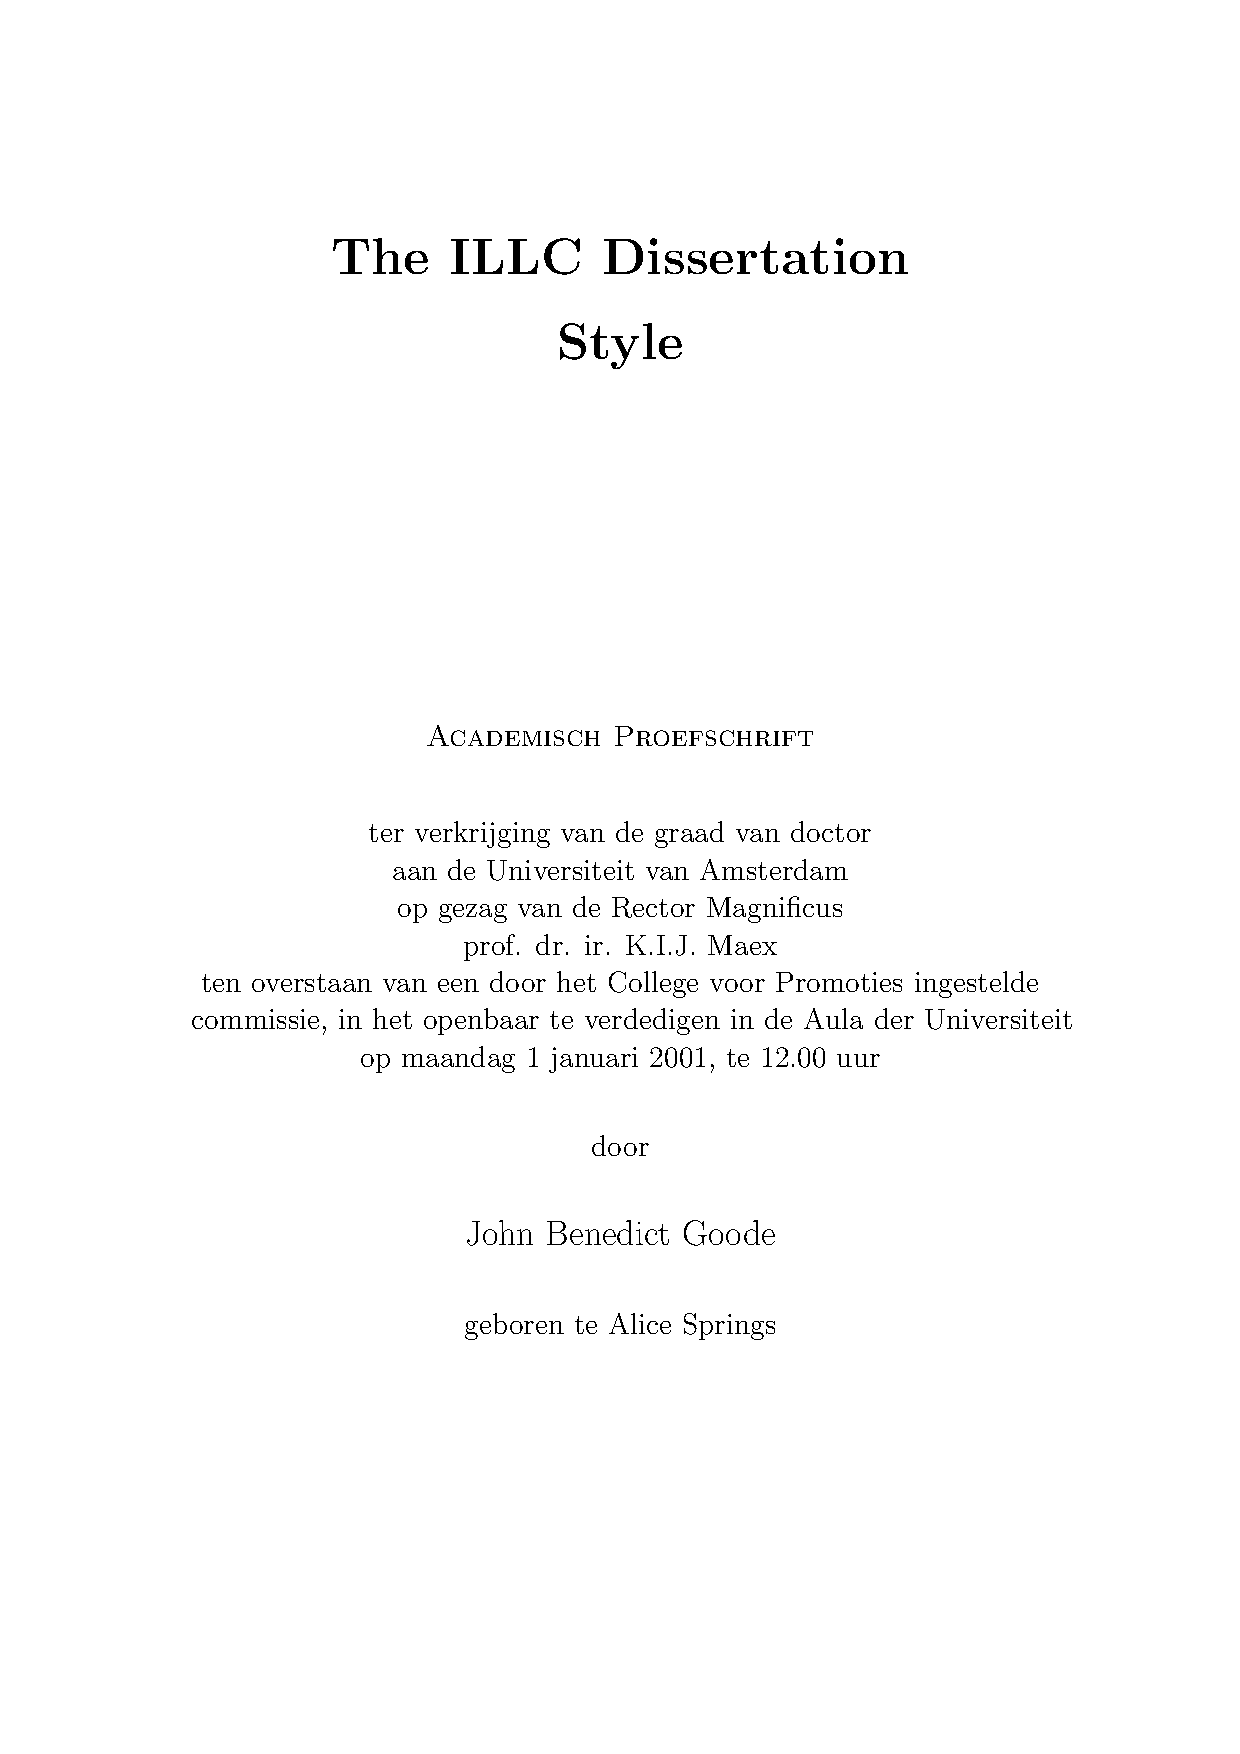
\includepdf[pages={1,2}]{titlepage_from_pedel.pdf}
%%Formerly the pages were generated by the following content
%  \par\vskip 2cm
%  \begin{center}
%  \printtitle
%  \par\vspace {6cm}
%  {\large \sc Academisch Proefschrift}
%  \par\vspace {1cm}
%  {\large ter verkrijging van de graad van doctor\\
%  aan de Universiteit van Amsterdam\\
%  op gezag van de Rector Magnificus\\
%  prof. dr. ir. K.I.J. Maex\\                                 %PERSONALIZE
%  ten overstaan van een door het College voor Promoties ingestelde\\
%  \mbox{commissie, in het openbaar te verdedigen in de Aula der Universiteit}\\        %PERSONALIZE
%  % Note: If your UvA PhD defense is located at the Agnietenkapel, simply write
%  % 'te verdedigen in de Agnietenkapel \\', i.e. do not add 'der Universiteit'
%  op maandag 1 januari 2001, te 12.00 uur \\ }        %PERSONALIZE
%  \par\vspace {1cm} {\large door}
%  \par \vspace {1cm} % Note: next should be your _full_ name
%  {\Large John Benedict Goode}                        %PERSONALIZE
%  \par\vspace {1cm} % and your birthplace
%  {\large geboren te Alice Springs} %PERSONALIZE
%  % Note: NEVER include your country of birth, only the city of birth
%  \end{center}
%  \clearpage
%  \noindent%
%  {\bfseries Promotiecommissie}\\
%  \\
%  \begin{tabular}[t]{@{}llr}
%  Promotor:      & Prof.dr.\ J.~Smith  & Universiteit van Amsterdam \\  %PERSONALIZE
%  Co-promotor:   & Dr.\ T.~Jones       & Universiteit van Amsterdam \\  %PERSONALIZE
%  \\
%  Overige leden: & Prof. Dr. A. Aap    & Universiteit van Amsterdam \\  %PERSONALIZE
%                 & Prof. Dr. B. Benson & Universiteit van Amsterdam \\  %PERSONALIZE
%                 & Dr. C. Cornelissen  & Universiteit van Amsterdam \\  %PERSONALIZE
%  \end{tabular}\\
%  \\
%  Faculteit der Natuurwetenschappen, Wiskunde en Informatica\\ %PERSONALIZE

\clearpage
} % Back to \pagestyle{plain}

%%%%%%%%%%%%%%%%%%%%%%%END of FRONT MATTER%%%%%%%%%%%%%%%%%%%%%%%%%%%

\thispagestyle{plain}
\mbox{}
\vspace{2in}
\begin{center}
{\em to me \\ \ \\
who did all the work on this}
\footnote{The dedication is optional}
\end{center}

\tableofcontents
\acknowledgments

I am very grateful to Prof.dr.\ J.\ Smith whose help proved really extremely
invaluable.\\[2ex]				
Alice Springs\hfill John B. Goode\\
October, 200X.



%%  now we can start with the real thing

\cleardoublepage
\pagestyle{headings}
\pagenumbering{arabic}

\chapter{Getting started}

This file describes the ILLC Dissertation Style package for
typesetting dissertations in \LaTeX\ according to ILLC standards.
It describes which files are needed, and how they should be adopted
for your dissertation.
It also serves as an example of using these files, and as a template
for your own dissertation.

The ILLC Dissertation Style file will change the
layout of your dissertation to the required ILLC Dissertation Style.
It defines a standard layout for the cover and spine of your dissertation,
and includes a list of previous publications in the ILLC Dissertation series
Furthermore, it redefines the layout of \verb|\chapter|, page heads,
and theorem-like environments,
and provides predefined theorem-like environments and
commands for special sections such as \verb|\acknowledgements|.

If you are already familiar with the standard {\tt book.cls} provided with
\LaTeX 2$\epsilon$, then the ILLC Dissertation Style file should not give you
any difficulties: you may use all {\tt book} style commands to prepare 
your dissertation.
For a description of the commands available in the \LaTeX 2$\epsilon$\ 
{\tt book} style we refer you to the {\em \LaTeX{} User's Guide \& Reference
Manual\/} by Leslie Lamport (1986, 1994), Addison-Wesley Publishing
Company, Reading, Mass.

\section{How to proceed}
The complete ILLC Dissertation Style package contains the following files:
\begin{description} 
\item[{\tt illcdiss.cls}:] the ILLC Dissertation Style for
use with \LaTeX 2$\epsilon$
\item[{\tt illcdissertations.tex}:] file containing data on previous
  ILLC Dissertations
\item[{\tt illclogo.eps}:] this is the ILLC logo;
  input by {\tt guide\_front.tex}
\item[{\tt illc\_no\_text\_logo.eps}:] the ILLC logo without text;
  input by {\tt guide\_spine.tex}
\item[{\tt illclogo.pdf}, {\tt illc\_no\_text\_logo.pdf}:] PDF versions of the logos, used by {\tt pdflatex} instead of the EPS versions
\item[{\tt guide.tex}:] the main latex file for this document
\item[{\tt guide\_front.tex}:] file describing the official 
  ILLC-Dissertation front matter
\item[{\tt titlepage\_from\_pedel.pdf}:] placeholder for the title page which you will receive from the Bureau Pedel (Office of the Beadle)
\item[{\tt guide\_XXX.tex}:] file containing the text of section XXX of this 
document
\item[{\tt guide\_spine.tex}:] file for preparing the text 
  for the spine of your dissertation
\end{description}
You should make sure that \LaTeX\ is able to find the files
{\tt illcdissertations.tex}, {\tt illcdiss.cls}, {\tt illclogo.eps} and
{\tt illc\_no\_text\_logo.eps} when you 
typeset your document with the ILLC Dissertation Style; one way
to achieve this is to put all files in the ILLC Dissertation Style
package in the directory (or folder) where your dissertation files
reside.

Note that the {\tt illcdissertations.tex}
file in the archive is automatically updated for any new dissertations:
please download the most recent version 
before sending your dissertation to the printers.

\section{Invoking the ILLC Dissertation Style}
The ILLC Dissertation Style is invoked by replacing ``book'' by ``illcdiss''
in the first line of your document. You should also \verb|\include| 
a {\em personalized\/} version of the file {\tt guide\_front.tex} 
after the \verb|\begin{document}| declaration. 
You also need to \verb|\include| the file
\verb|illcdissertations.tex| after the last page of your dissertation:

\begin{verbatim}
\documentclass{illcdiss}

\begin{document}
\pagestyle{plain}
\pagenumbering{roman}

%%  \include the `front matter'

%% This is the standard `front matter' to be used with the illcdiss.cls
%% Latex2e document class
%%
%% Author: Maarten de Rijke
%% Current maintainer: Marco Vervoort
%%
%% Version: July, 2001
%%
%%
%% Amendment August, 2020 by Gianluca Grilletti: the nationality of the candidate should not be indicated in the titelblad, independently from the birth country
%%
%%
%%
%% MAKE SURE THAT THE FILE HAS BEEN PERSONALIZED BEFORE YOU
%% PRINT AND SHIP THE FINAL VERSION.  YOU CAN FIND ITEMS THAT NEED
%% TO BE PERSONALIZED BY SEARCHING FOR THE STRING ``%PERSONALIZE''
%%
%%
%%first of all the cover.
{\pagestyle{empty}
\newcommand{\printtitle}{%
{\Huge\bfseries The ILLC Dissertation\\[0.8cm] Style}}    %PERSONALIZE

\begin{titlepage}
\par\vskip 2cm
\begin{center}
\printtitle
\vfill
{\LARGE\bfseries John B. Goode}                           %PERSONALIZE
\vskip 2cm
\end{center}
\end{titlepage}
%
% Skip a page to start on a right page again.
% If you're printing single-sided, simply delete    %PERSONALIZE
% the following line.
%
\mbox{}\newpage
\setcounter{page}{1}

%%the very first page: the `franse pagina'
\par\vskip 2cm
\begin{center}
\printtitle
\end{center}

%%the second page: the `illc pagina'
\clearpage
\par\vskip 2cm
\begin{center}
ILLC Dissertation Series DS-200X-NN                 %PERSONALIZE
\par\vspace {2cm}
\illclogo{10cm}
\par\vspace {2cm}
\noindent%
For further information about ILLC-publications, please contact\\[2ex]
Institute for Logic, Language and Computation\\
Universiteit van Amsterdam\\
Science Park 107\\
1098 XG Amsterdam\\
phone: +31-20-525 6051\\
e-mail: {\tt illc@uva.nl}\\
homepage: {\tt http://www.illc.uva.nl/}
\end{center}
\vfill

% If you're supported by NWO adapt the following 6 lines;
% otherwise simply delete them.
%
\noindent%
The investigations were supported by the            %PERSONALIZE
Philosophy Research Foundation\linebreak (SWON), 
which is subsidized by the Netherlands 
Organization for Scientific\linebreak Research (NWO).
\par\vspace {2cm}

% If you want to add CIP data (a summary of all the data used in
% library catalogs in a standard format), uncomment the following
% three lines and add the CIP data in between
%
%\noindent%
%{\tt CIP gegevens}                                 % PERSONALIZE
%\\[4ex]                                            %PERSONALIZE

%Copyright and accreditation stuff, plus ISBN
%
\noindent%
% Copyright: put your name here
Copyright \copyright\ 200X by John B.\ Goode\\[2ex] %PERSONALIZE
% Cover design, if your cover was designed by someone else
Cover design by Bert Jones.\\                       %PERSONALIZE
%Maybe some additional info on the production of the dissertation.
%Don't forget your printing shop
Printed and bound by your printer.\\[2ex]           %PERSONALIZE
%ISBN number: ask your printing shop to obtain one for you
ISBN: 90--XXXX--XXX--X                              %PERSONALIZE

% Dedication, table of contents and acknowledgements
% are handled in the main file


%%the third and fourth page, the `titelblad' and promotores-list, will be sent to you by the Pedel. Replace the file 'titlepage_from_pedel.pdf' by what you receive.
\clearpage
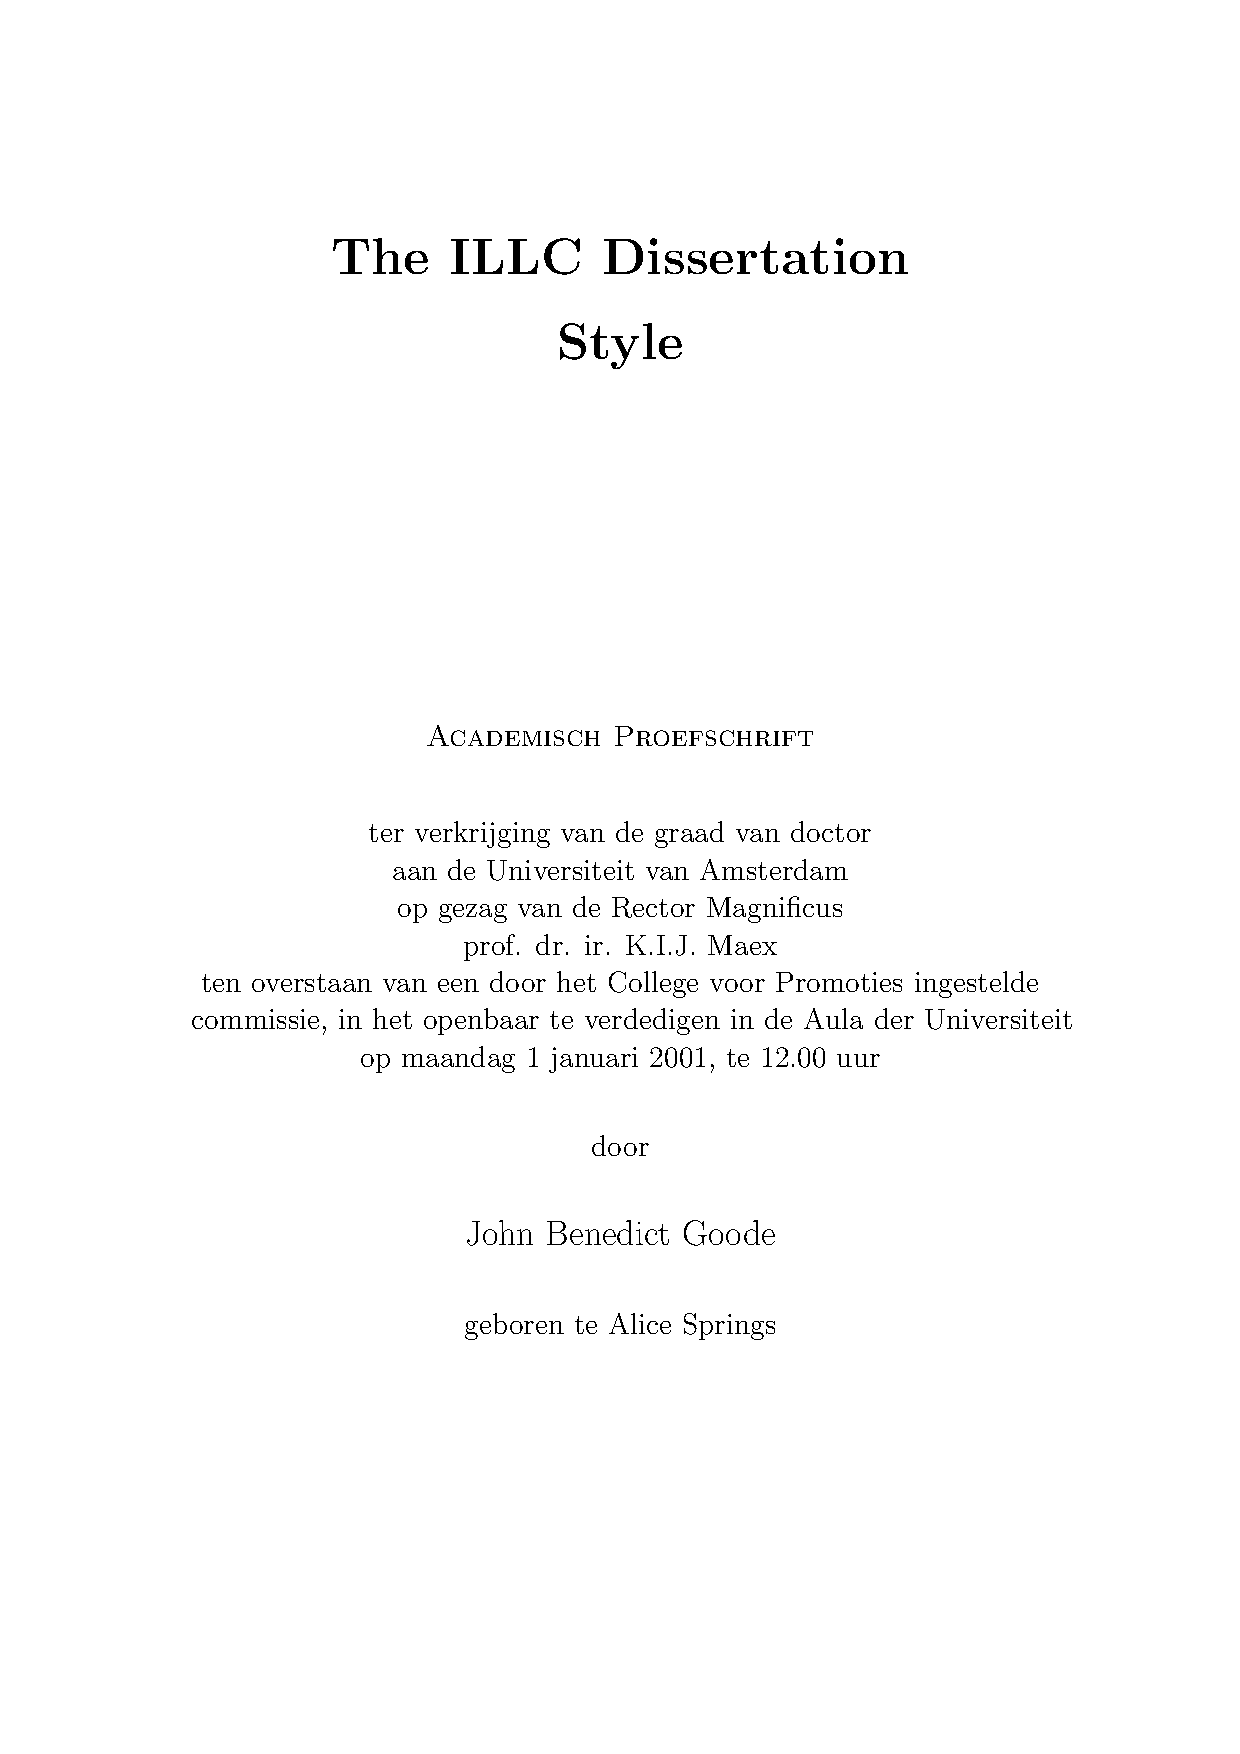
\includepdf[pages={1,2}]{titlepage_from_pedel.pdf}
%%Formerly the pages were generated by the following content
%  \par\vskip 2cm
%  \begin{center}
%  \printtitle
%  \par\vspace {6cm}
%  {\large \sc Academisch Proefschrift}
%  \par\vspace {1cm}
%  {\large ter verkrijging van de graad van doctor\\
%  aan de Universiteit van Amsterdam\\
%  op gezag van de Rector Magnificus\\
%  prof. dr. ir. K.I.J. Maex\\                                 %PERSONALIZE
%  ten overstaan van een door het College voor Promoties ingestelde\\
%  \mbox{commissie, in het openbaar te verdedigen in de Aula der Universiteit}\\        %PERSONALIZE
%  % Note: If your UvA PhD defense is located at the Agnietenkapel, simply write
%  % 'te verdedigen in de Agnietenkapel \\', i.e. do not add 'der Universiteit'
%  op maandag 1 januari 2001, te 12.00 uur \\ }        %PERSONALIZE
%  \par\vspace {1cm} {\large door}
%  \par \vspace {1cm} % Note: next should be your _full_ name
%  {\Large John Benedict Goode}                        %PERSONALIZE
%  \par\vspace {1cm} % and your birthplace
%  {\large geboren te Alice Springs} %PERSONALIZE
%  % Note: NEVER include your country of birth, only the city of birth
%  \end{center}
%  \clearpage
%  \noindent%
%  {\bfseries Promotiecommissie}\\
%  \\
%  \begin{tabular}[t]{@{}llr}
%  Promotor:      & Prof.dr.\ J.~Smith  & Universiteit van Amsterdam \\  %PERSONALIZE
%  Co-promotor:   & Dr.\ T.~Jones       & Universiteit van Amsterdam \\  %PERSONALIZE
%  \\
%  Overige leden: & Prof. Dr. A. Aap    & Universiteit van Amsterdam \\  %PERSONALIZE
%                 & Prof. Dr. B. Benson & Universiteit van Amsterdam \\  %PERSONALIZE
%                 & Dr. C. Cornelissen  & Universiteit van Amsterdam \\  %PERSONALIZE
%  \end{tabular}\\
%  \\
%  Faculteit der Natuurwetenschappen, Wiskunde en Informatica\\ %PERSONALIZE

\clearpage
} % Back to \pagestyle{plain}

%%%%%%%%%%%%%%%%%%%%%%%END of FRONT MATTER%%%%%%%%%%%%%%%%%%%%%%%%%%%

\thispagestyle{plain}
\mbox{}
\vspace{2in}
\begin{center}
{\em to me \\ \ \\
who did all the work on this}
\footnote{The dedication is optional}
\end{center}

\tableofcontents
\acknowledgments

I am very grateful to Prof.dr.\ J.\ Smith whose help proved really extremely
invaluable.\\[2ex]				
Alice Springs\hfill John B. Goode\\
October, 200X.



%%  now we can start with the real thing

\cleardoublepage
\pagestyle{headings}
\pagenumbering{arabic}
  
    <your dissertation>

%%  \include the `end matter'

% \begin{thebibliography}{XX}
% \bibitem{Comment}
% According to ILLC standards a chapter containing bibliographic
% references should always be included in your dissertation.
% It is specified by:
% \begin{verbatim}
%   \begin{thebibliography}{XX}
%     <your list of \bibitems>
%   \end{thebibliography}
% \end{verbatim}
% \bibitem{Lamport}
% L. Lamport. {\em \LaTeX{} User's Guide \& Reference
% Manual\/}, Addison-Wesley Publishing Company, Reading, Mass. 1986, 1994.
% \end{thebibliography}

\bibliography{biblio}


\begin{theindex}
By preference, your dissertation\linebreak
should contain an index. Instructions
on how to produce an index can be
found on pages 77--79 of the
 \LaTeX\ manual. You may specify
an index as follows:\\[2ex]
\verb|  \begin{theindex}|\\
\verb|    <your list of entries>|\\
\verb|  \end{theindex}|
\end{theindex}


\begin{thesymbols}
This is an optional chapter containing a list of symbols that
you use. It is specified by:\\[2ex]
\verb|  \begin{thesymbols}|\\
\verb|    <your list of symbols>|\\
\verb|  \end{thesymbols}|
\end{thesymbols}

\samenvatting
According to both ILLC standards and UvA promotion regulations,
a chapter containing a summary in
Dutch of your dissertation should always be included.
It is specified by:
\begin{verbatim}
  \samenvatting
    <your Samenvatting>
\end{verbatim}

\abstract
According to both ILLC standards and UvA promotion regulations,
an abstract of your dissertation in English should always be included.
This chapter may be specified by:
\begin{verbatim}
  \abstract
    <your Abstract>
\end{verbatim}


\curriculum
This is an optional chapter containing your Curriculum Vitae.
It is specified as follows:
\begin{verbatim}
  \curriculum
    <your CV>
\end{verbatim}



%%  finally, \include the list of previous ILLC dissertations

\pagestyle{empty}

\noindent
{\em Titles in the ILLC Dissertation Series:}

\newcommand{\illcpublication}[3]{\item[ILLC #1: ]{\bfseries #2}\\{\em #3}}

\begin{list}{}{ \settowidth{\leftmargin}{ILL}
		\setlength{\rightmargin}{0in}
		\setlength{\labelwidth}{\leftmargin}
		\setlength{\labelsep}{0in}
}

\illcpublication{DS-2016-01}{Ivano A. Ciardelli}{Questions in Logic}
\illcpublication{DS-2016-02}{Zoé Christoff}{Dynamic Logics of Networks: Information Flow and the Spread of Opinion}
\illcpublication{DS-2016-03}{Fleur Leonie Bouwer}{What do we need to hear a beat? The influence of attention, musical abilities, and accents on the perception of metrical rhythm}
\illcpublication{DS-2016-04}{Johannes Marti}{Interpreting Linguistic Behavior with Possible World Models}
\illcpublication{DS-2016-05}{Phong Lê}{Learning Vector Representations for Sentences - The Recursive Deep Learning Approach}
\illcpublication{DS-2016-06}{Gideon Maillette de Buy Wenniger}{Aligning the Foundations of Hierarchical Statistical Machine Translation}
\illcpublication{DS-2016-07}{Andreas van Cranenburgh}{Rich Statistical Parsing and Literary Language}
\illcpublication{DS-2016-08}{Florian Speelman}{Position-based Quantum Cryptography and Catalytic Computation}
\illcpublication{DS-2016-09}{Teresa Piovesan}{Quantum entanglement: insights via graph parameters and conic optimization}
\illcpublication{DS-2016-10}{Paula Henk}{Nonstandard Provability for Peano Arithmetic. A Modal Perspective}
\illcpublication{DS-2017-01}{Paolo Galeazzi}{Play Without Regret}
\illcpublication{DS-2017-02}{Riccardo Pinosio}{The Logic of Kant's Temporal Continuum}
\illcpublication{DS-2017-03}{Matthijs Westera}{Exhaustivity and intonation: a unified theory}
\illcpublication{DS-2017-04}{Giovanni Cinà}{Categories for the working modal logician}
\illcpublication{DS-2017-05}{Shane Noah Steinert-Threlkeld}{Communication and Computation: New Questions About Compositionality}
\illcpublication{DS-2017-06}{Peter Hawke}{The Problem of Epistemic Relevance}
\illcpublication{DS-2017-07}{Aybüke Özgün}{Evidence in Epistemic Logic: A Topological Perspective}
\illcpublication{DS-2017-08}{Raquel Garrido Alhama}{Computational Modelling of Artificial Language Learning: Retention, Recognition \& Recurrence}
\illcpublication{DS-2017-09}{Miloš Stanojević}{Permutation Forests for Modeling Word Order in Machine Translation}
\illcpublication{DS-2018-01}{Berit Janssen}{Retained or Lost in Transmission? Analyzing and Predicting Stability in Dutch Folk Songs}
\illcpublication{DS-2018-02}{Hugo Huurdeman}{Supporting the Complex Dynamics of the Information Seeking Process}
\illcpublication{DS-2018-03}{Corina Koolen}{Reading beyond the female: The relationship between perception of author gender and literary quality}
\illcpublication{DS-2018-04}{Jelle Bruineberg}{Anticipating Affordances: Intentionality in self-organizing brain-body-environment systems}
\illcpublication{DS-2018-05}{Joachim Daiber}{Typologically Robust Statistical Machine Translation: Understanding and Exploiting Differences and Similarities Between Languages in Machine Translation}
\illcpublication{DS-2018-06}{Thomas Brochhagen}{Signaling under Uncertainty}
\illcpublication{DS-2018-07}{Julian Schlöder}{Assertion and Rejection}
\illcpublication{DS-2018-08}{Srinivasan Arunachalam}{Quantum Algorithms and Learning Theory}
\illcpublication{DS-2018-09}{Hugo de Holanda Cunha Nobrega}{Games for functions: Baire classes, Weihrauch degrees, transfinite computations, and ranks}
\illcpublication{DS-2018-10}{Chenwei Shi}{Reason to Believe}
\illcpublication{DS-2018-11}{Malvin Gattinger}{New Directions in Model Checking Dynamic Epistemic Logic}
\illcpublication{DS-2018-12}{Julia Ilin}{Filtration Revisited: Lattices of Stable Non-Classical Logics}
\illcpublication{DS-2018-13}{Jeroen Zuiddam}{Algebraic complexity, asymptotic spectra and entanglement polytopes}
\illcpublication{DS-2019-01}{Carlos Vaquero}{What Makes A Performer Unique? Idiosyncrasies and commonalities in expressive music performance}
\illcpublication{DS-2019-02}{Jort Bergfeld}{Quantum logics for expressing and proving the correctness of quantum programs}
\illcpublication{DS-2019-03}{András Gilyén}{Quantum Singular Value Transformation \& Its Algorithmic Applications}
\illcpublication{DS-2019-04}{Lorenzo Galeotti}{The theory of the generalised real numbers and other topics in logic}
\illcpublication{DS-2019-05}{Nadine Theiler}{Taking a unified perspective: Resolutions and highlighting in the semantics of attitudes and particles}
\illcpublication{DS-2019-06}{Peter T.S. van der Gulik}{Considerations in Evolutionary Biochemistry}
\illcpublication{DS-2019-07}{Frederik Möllerström Lauridsen}{Cuts and Completions: Algebraic aspects of structural proof theory}
\illcpublication{DS-2020-01}{Mostafa Dehghani}{Learning with Imperfect Supervision for Language Understanding}
\illcpublication{DS-2020-02}{Koen Groenland}{Quantum protocols for few-qubit devices}
\illcpublication{DS-2020-03}{Jouke Witteveen}{Parameterized Analysis of Complexity}
\illcpublication{DS-2020-04}{Joran van Apeldoorn}{A Quantum View on Convex Optimization}
\illcpublication{DS-2020-05}{Tom Bannink}{Quantum and stochastic processes}
\illcpublication{DS-2020-06}{Dieuwke Hupkes}{Hierarchy and interpretability in neural models of language processing}
\illcpublication{DS-2020-07}{Ana Lucia Vargas Sandoval}{On the Path to the Truth: Logical \& Computational Aspects of Learning}
\illcpublication{DS-2020-08}{Philip Schulz}{Latent Variable Models for Machine Translation and How to Learn Them}
\illcpublication{DS-2020-09}{Jasmijn Bastings}{A Tale of Two Sequences: Interpretable and Linguistically-Informed Deep Learning for Natural Language Processing}
\illcpublication{DS-2020-10}{Arnold Kochari}{Perceiving and communicating magnitudes: Behavioral and electrophysiological studies}
\illcpublication{DS-2020-11}{Marco Del Tredici}{Linguistic Variation in Online Communities: A Computational Perspective}
\illcpublication{DS-2020-12}{Bastiaan van der Weij}{Experienced listeners: Modeling the influence of long-term musical exposure on rhythm perception}
\illcpublication{DS-2020-13}{Thom van Gessel}{Questions in Context}
\illcpublication{DS-2020-14}{Gianluca Grilletti}{Questions \& Quantification: A study of first order inquisitive logic}
\illcpublication{DS-2020-15}{Tom Schoonen}{Tales of Similarity and Imagination. A modest epistemology of possibility}
\illcpublication{DS-2020-16}{Ilaria Canavotto}{Where Responsibility Takes You: Logics of Agency, Counterfactuals and Norms}
\illcpublication{DS-2020-17}{Francesca Zaffora Blando}{Patterns and Probabilities: A Study in Algorithmic Randomness and Computable Learning}
\illcpublication{DS-2021-01}{Yfke Dulek}{Delegated and Distributed Quantum Computation}
\illcpublication{DS-2021-02}{Elbert J. Booij}{The Things Before Us: On What it Is to Be an Object}
\illcpublication{DS-2021-03}{Seyyed Hadi Hashemi}{Modeling Users Interacting with Smart Devices}
\illcpublication{DS-2021-04}{Sophie Arnoult}{Adjunction in Hierarchical Phrase-Based Translation}
\illcpublication{DS-2021-05}{Cian Guilfoyle Chartier}{A Pragmatic Defense of Logical Pluralism}
\illcpublication{DS-2021-06}{Zoi Terzopoulou}{Collective Decisions with Incomplete Individual Opinions}
\illcpublication{DS-2021-07}{Anthia Solaki}{Logical Models for Bounded Reasoners}
\illcpublication{DS-2021-08}{Michael Sejr Schlichtkrull}{Incorporating Structure into Neural Models for Language Processing}
\illcpublication{DS-2021-09}{Taichi Uemura}{Abstract and Concrete Type Theories}
\illcpublication{DS-2021-10}{Levin Hornischer}{Dynamical Systems via Domains: Toward a Unified Foundation of Symbolic and Non-symbolic Computation}

\end{list}

\end{document}
\end{verbatim}
%
%
If your file is already coded with \LaTeX{} you can easily
adapt it a posteriori to the ILLC Dissertation Style.

If your document is coded with the ILLC Dissertation Style,
you may not be able to typeset it using the standard \LaTeX\ book style
without doing some minor recoding,
as the ILLC Dissertation Style file defines some comands 
that are not provided by the standard \LaTeX\ book style.

Please refrain from using any \LaTeX{} or \TeX{} commands
that affect the layout or formatting of your document
(i.e.\ commands like \verb|\textheight|, \verb|\hoffset| etc.).
The ILLC Dissertation Style has been carefully designed 
to produce the rightlayout from your \LaTeX\ input.
There may nevertheless be exceptional occasions on which to use some of them.
If there is anything specific you would like to do 
and for which neither \LaTeX{} nor the ILLC Dissertation Style file 
provides a command,
{\em please contact us\/} (email: illc@uva.nl).

\section{Personalizing {\tt guide\_front.tex}}
The file {\tt guide\_front.tex} contains all information needed 
to produce the front matter of your dissertation according to ILLC standards.
You need to personalize {\tt guide\_front.tex} by inserting your data
at appropriate spots. Additionally, those that print on single-sided
printers will want to eliminate the empty page printed after the cover page.
All items that need to be personalized in 
{\tt guide\_front.tex} can be found by searching for the string 
``\%{}PERSONALIZE''.

You will receive a version containing a title page from the Bureau Pedel (Office of the Beadle) once your dissertation has been approved by the committee.
This should be included as pages (iii) and (iv) of the front matter, using the pdfpages \verb|\includepdf| command.
An example file 'titlepage\_from\_pedel.pdf' is included with the style files.
Note that you may wish to temporarily comment out the \verb|\includepdf| command for the version that is sent to your committee, as at that point you will not yet have obtained the proper title page and the example file will list the wrong title.

The files {\tt guide\_dedication} and {\tt guide\_acknowledgements} 
contain the optional dedication and acknowledgements, and are \verb|\include|d
from the main file.
You can personalize the text in these files, or simply change the name
of the \verb|\include|d files in the main file.

\section{Personalizing {\tt guide\_spine.tex}}
The file {\tt guide\_spine.tex} contains all information needed
to produce the spine of your dissertation according to ILLC standards.
You need to personalize the file {\tt guide\_spine.tex} by inserting 
your data at appropriate spots. All items that need to be personalized in
{\tt guide\_spine.tex} can be found by searching for the string
``\%{}PERSONALIZE''.

\chapter{The order of things}
According to ILLC standards your dissertation should meet a limited number
of requirements concerning its organization and layout. You need hardly 
worry about details concerning the layout as these are handled by the
ILLC Dissertation Style file. The following describes how your dissertation
should be organized.

\section{The cover}
The ILLC Dissertation Style only prescribes the font, size and location 
of the title and author on the cover page. Besides this you are free to 
design your own cover.

Dissertations formatted according to ILLC standards have a spine displaying
the authors name, the title of the dissertation, and the ILLC logo.
There is a file called {\tt guide\_spine.tex} to help you format 
your spine text.


\section{The front matter}
The front matter has Roman page numbers (this is achieved by
specifying the command \verb|\pagenumbering{roman}| after the 
\verb|\begin{document}| declaration). The front matter should contain 
the following material in the following order:
\begin{enumerate}
\item[i]
``franse pagina'' containing nothing but the title of your dissertation
\item[ii]
the ``ILLC page'' containing the logo and address of ILLC
\item[iii]
the title page containing the text prescribed by the university
\item[iv]
this page contains the following information in the following order:
	\begin{itemize}
	\item
	name and address of your promotor (es)
	\item
	when appropriate, an acknowledgment to NWO or its subfoundations
	\item
	CIP-gegevens (optional), cataloguing data for the National Library
	\item
	a copyright notice
	\item
	information concerning the production of your dissertation
	\item
	the ISBN code
	\end{itemize}
\item[v] (optional)
dedication
\item[v] (or vii)
table of contents
\item[vii] (or ix)
Acknowledgments, specified by \verb|\acknowledgments|.
\end{enumerate}
The file called  \verb|guide_front.tex| helps you format
the front matter of your dissertation.
Pages (iii) and (iv) will be sent to you by the Bureau Pedel (Office of the Beadle).



\section{The body of your text}
This section contains some information about organizing the main
text of your dissertation.

\paragraph*{Headings.}
Headings will be automatically generated by the following codes
\begin{verbatim}
  \chapter
  \section
  \subsection
  \subsubsection
  \paragraph
\end{verbatim}
The headings produced by \verb|\paragraph| and \verb|\subparagraph| 
need to be punctuated at the end,
as they are followed by the body of the (sub-)paragraph.

\paragraph*{Theorem-like environments.}
In addition to the above headings your text may be structured 
by theorem-like environments, like lemmas, propositions, conjectures, \ldots .
The following theorem-like environments are predefined by the ILLC Disseration 
Style file: \verb|theorem|, \verb|lemma|, \verb|corollary|, \verb|conjecture|, 
\verb|proposition|, \verb|definition|, \verb|remark|, 
\verb|example|, \verb|convention|, \verb|fact| and \verb|question|.
They are defined to be numbered consecutively, i.e. typing
\begin{verbatim}
\begin{lemma}
This is a lemma
\end{lemma}
\begin{proof}
This is a proof\\
With two lines
\end{proof}
\begin{question}
Is this a question?
\end{question}
\end{verbatim}
produces
\begin{lemma}
This is a lemma
\end{lemma}
\begin{proof}
This is a proof\\
With two lines
\end{proof}
\begin{question}
Is this a question?
\end{question}

A number of theorem-like environments have italicized text:
\verb|theorem|, \verb|lemma|, \verb|corollary|, \verb|conjecture|
and \verb|proposition|. All other pre-defined environments have roman text.
Inside theorem-like environments text may be emphasized by
using \verb|\em|. (In environments with italicized text such as lemma
and theorems this will produce text in roman type style; in 
environments with roman text this produces italicized text.)
As a rule of thumb you should always emphasize the terms being
defined in a definition.

\paragraph*{Special signs and characters.}
\newcommand{\AmSTeX}{%
{$\cal A$}\kern-.1667em\lower.5ex\hbox
  {$\cal M$}\kern-.125em{$\cal S$}-\TeX
}
You may need to use special signs. The available ones are listed
in the \LaTeX{} {\em User's Guide \& Reference Manual\/}, pp.~44 ff.
If you need other symbols than those, you could use the symbols
of the \AmSTeX{} fonts. The  \AmSTeX{} fonts also contain gothic letters
and `blackboard bold' characters such as ${\rm I}\hskip -.3pt{\rm N}$. Consult
your local \TeX{} wizzard for instructions on using the \AmSTeX{} fonts.

\paragraph*{Splitting your input}
Rather than putting the whole input of a document in a single file, you
may wish to split it into several smaller ones.
There will always be one file that is the {\em root} file; it is the one
whose name you type when you run \LaTeX{}.
The root file of the document you are reading is called \verb|guide.tex|.
Other files may be `included' by the commands \verb|\input| and \verb|\include|.
The command \verb|\input{filename}| causes \LaTeX{} to insert the contents
of the file \verb|filename.tex| right at the current spot in your manuscript.
The command \verb|\include{filename}| does the same, except that the
included text will begin and end on its own page (i.e. an automatic
\verb|\clearpage| command is issued at the beginning and end of the included
file).
Additionally, this allows the use of the \verb|\includeonly| command
(see the paragraph on saving paper).
The \verb|\include| command is the preferred way to include a file containing,
for instance, the text of a single chapter.

\section{The end matter}
The end matter should at least contain a Bibliography, a Samenvatting,
an Abstract
and a list of previous publications in the ILLC Dissertation Series.
Note that both a dutch summary and an english abstract are obligatory
in english dissertations, according to UvA promotion regulations.
Preferably your dissertation also contains an Index.
In addition it may contain
Appendices, a List of Symbols and your Curriculum Vitae. According to ILLC
standards the material should be included in the following order:
\begin{itemize}
\item
Appendices (optional), see pp.\ 23, 158 of the
  \LaTeX{} {\em User's Guide \& Reference Manual\/} on how to create
  appendices 
\item
Bibliography (obligatory), specified by 
\begin{verbatim}
  \begin{thebibliography}{XX}
    <your list of \bibitems>
  \end{thebibliography}
\end{verbatim}
\item
Index, specified by
\begin{verbatim}
  \begin{theindex}
    <your list of entries>
  \end{theindex}
\end{verbatim}
\item
List of Symbols (optional), specified by
\begin{verbatim}
  \begin{thesymbols}
    <your list of symbols>
  \end{thesymbols}
\end{verbatim}
\item
Samenvatting (obligatory), specified by
\begin{verbatim}
  \samenvatting
    <your Samenvatting>
\end{verbatim}
\item
Abstract (obligatory), specified by
\begin{verbatim}
  \abstract
    <your Abstract>
\end{verbatim}

\item
Curriculum Vitae (optional), specified by
\begin{verbatim}
  \curriculum
    <your CV>
\end{verbatim}
\item
List of previous publications in the ILLC Dissertation Series (obligatory), 
specified by
\begin{verbatim}
  \pagestyle{empty}

\noindent
{\em Titles in the ILLC Dissertation Series:}

\newcommand{\illcpublication}[3]{\item[ILLC #1: ]{\bfseries #2}\\{\em #3}}

\begin{list}{}{ \settowidth{\leftmargin}{ILL}
		\setlength{\rightmargin}{0in}
		\setlength{\labelwidth}{\leftmargin}
		\setlength{\labelsep}{0in}
}

\illcpublication{DS-2016-01}{Ivano A. Ciardelli}{Questions in Logic}
\illcpublication{DS-2016-02}{Zoé Christoff}{Dynamic Logics of Networks: Information Flow and the Spread of Opinion}
\illcpublication{DS-2016-03}{Fleur Leonie Bouwer}{What do we need to hear a beat? The influence of attention, musical abilities, and accents on the perception of metrical rhythm}
\illcpublication{DS-2016-04}{Johannes Marti}{Interpreting Linguistic Behavior with Possible World Models}
\illcpublication{DS-2016-05}{Phong Lê}{Learning Vector Representations for Sentences - The Recursive Deep Learning Approach}
\illcpublication{DS-2016-06}{Gideon Maillette de Buy Wenniger}{Aligning the Foundations of Hierarchical Statistical Machine Translation}
\illcpublication{DS-2016-07}{Andreas van Cranenburgh}{Rich Statistical Parsing and Literary Language}
\illcpublication{DS-2016-08}{Florian Speelman}{Position-based Quantum Cryptography and Catalytic Computation}
\illcpublication{DS-2016-09}{Teresa Piovesan}{Quantum entanglement: insights via graph parameters and conic optimization}
\illcpublication{DS-2016-10}{Paula Henk}{Nonstandard Provability for Peano Arithmetic. A Modal Perspective}
\illcpublication{DS-2017-01}{Paolo Galeazzi}{Play Without Regret}
\illcpublication{DS-2017-02}{Riccardo Pinosio}{The Logic of Kant's Temporal Continuum}
\illcpublication{DS-2017-03}{Matthijs Westera}{Exhaustivity and intonation: a unified theory}
\illcpublication{DS-2017-04}{Giovanni Cinà}{Categories for the working modal logician}
\illcpublication{DS-2017-05}{Shane Noah Steinert-Threlkeld}{Communication and Computation: New Questions About Compositionality}
\illcpublication{DS-2017-06}{Peter Hawke}{The Problem of Epistemic Relevance}
\illcpublication{DS-2017-07}{Aybüke Özgün}{Evidence in Epistemic Logic: A Topological Perspective}
\illcpublication{DS-2017-08}{Raquel Garrido Alhama}{Computational Modelling of Artificial Language Learning: Retention, Recognition \& Recurrence}
\illcpublication{DS-2017-09}{Miloš Stanojević}{Permutation Forests for Modeling Word Order in Machine Translation}
\illcpublication{DS-2018-01}{Berit Janssen}{Retained or Lost in Transmission? Analyzing and Predicting Stability in Dutch Folk Songs}
\illcpublication{DS-2018-02}{Hugo Huurdeman}{Supporting the Complex Dynamics of the Information Seeking Process}
\illcpublication{DS-2018-03}{Corina Koolen}{Reading beyond the female: The relationship between perception of author gender and literary quality}
\illcpublication{DS-2018-04}{Jelle Bruineberg}{Anticipating Affordances: Intentionality in self-organizing brain-body-environment systems}
\illcpublication{DS-2018-05}{Joachim Daiber}{Typologically Robust Statistical Machine Translation: Understanding and Exploiting Differences and Similarities Between Languages in Machine Translation}
\illcpublication{DS-2018-06}{Thomas Brochhagen}{Signaling under Uncertainty}
\illcpublication{DS-2018-07}{Julian Schlöder}{Assertion and Rejection}
\illcpublication{DS-2018-08}{Srinivasan Arunachalam}{Quantum Algorithms and Learning Theory}
\illcpublication{DS-2018-09}{Hugo de Holanda Cunha Nobrega}{Games for functions: Baire classes, Weihrauch degrees, transfinite computations, and ranks}
\illcpublication{DS-2018-10}{Chenwei Shi}{Reason to Believe}
\illcpublication{DS-2018-11}{Malvin Gattinger}{New Directions in Model Checking Dynamic Epistemic Logic}
\illcpublication{DS-2018-12}{Julia Ilin}{Filtration Revisited: Lattices of Stable Non-Classical Logics}
\illcpublication{DS-2018-13}{Jeroen Zuiddam}{Algebraic complexity, asymptotic spectra and entanglement polytopes}
\illcpublication{DS-2019-01}{Carlos Vaquero}{What Makes A Performer Unique? Idiosyncrasies and commonalities in expressive music performance}
\illcpublication{DS-2019-02}{Jort Bergfeld}{Quantum logics for expressing and proving the correctness of quantum programs}
\illcpublication{DS-2019-03}{András Gilyén}{Quantum Singular Value Transformation \& Its Algorithmic Applications}
\illcpublication{DS-2019-04}{Lorenzo Galeotti}{The theory of the generalised real numbers and other topics in logic}
\illcpublication{DS-2019-05}{Nadine Theiler}{Taking a unified perspective: Resolutions and highlighting in the semantics of attitudes and particles}
\illcpublication{DS-2019-06}{Peter T.S. van der Gulik}{Considerations in Evolutionary Biochemistry}
\illcpublication{DS-2019-07}{Frederik Möllerström Lauridsen}{Cuts and Completions: Algebraic aspects of structural proof theory}
\illcpublication{DS-2020-01}{Mostafa Dehghani}{Learning with Imperfect Supervision for Language Understanding}
\illcpublication{DS-2020-02}{Koen Groenland}{Quantum protocols for few-qubit devices}
\illcpublication{DS-2020-03}{Jouke Witteveen}{Parameterized Analysis of Complexity}
\illcpublication{DS-2020-04}{Joran van Apeldoorn}{A Quantum View on Convex Optimization}
\illcpublication{DS-2020-05}{Tom Bannink}{Quantum and stochastic processes}
\illcpublication{DS-2020-06}{Dieuwke Hupkes}{Hierarchy and interpretability in neural models of language processing}
\illcpublication{DS-2020-07}{Ana Lucia Vargas Sandoval}{On the Path to the Truth: Logical \& Computational Aspects of Learning}
\illcpublication{DS-2020-08}{Philip Schulz}{Latent Variable Models for Machine Translation and How to Learn Them}
\illcpublication{DS-2020-09}{Jasmijn Bastings}{A Tale of Two Sequences: Interpretable and Linguistically-Informed Deep Learning for Natural Language Processing}
\illcpublication{DS-2020-10}{Arnold Kochari}{Perceiving and communicating magnitudes: Behavioral and electrophysiological studies}
\illcpublication{DS-2020-11}{Marco Del Tredici}{Linguistic Variation in Online Communities: A Computational Perspective}
\illcpublication{DS-2020-12}{Bastiaan van der Weij}{Experienced listeners: Modeling the influence of long-term musical exposure on rhythm perception}
\illcpublication{DS-2020-13}{Thom van Gessel}{Questions in Context}
\illcpublication{DS-2020-14}{Gianluca Grilletti}{Questions \& Quantification: A study of first order inquisitive logic}
\illcpublication{DS-2020-15}{Tom Schoonen}{Tales of Similarity and Imagination. A modest epistemology of possibility}
\illcpublication{DS-2020-16}{Ilaria Canavotto}{Where Responsibility Takes You: Logics of Agency, Counterfactuals and Norms}
\illcpublication{DS-2020-17}{Francesca Zaffora Blando}{Patterns and Probabilities: A Study in Algorithmic Randomness and Computable Learning}
\illcpublication{DS-2021-01}{Yfke Dulek}{Delegated and Distributed Quantum Computation}
\illcpublication{DS-2021-02}{Elbert J. Booij}{The Things Before Us: On What it Is to Be an Object}
\illcpublication{DS-2021-03}{Seyyed Hadi Hashemi}{Modeling Users Interacting with Smart Devices}
\illcpublication{DS-2021-04}{Sophie Arnoult}{Adjunction in Hierarchical Phrase-Based Translation}
\illcpublication{DS-2021-05}{Cian Guilfoyle Chartier}{A Pragmatic Defense of Logical Pluralism}
\illcpublication{DS-2021-06}{Zoi Terzopoulou}{Collective Decisions with Incomplete Individual Opinions}
\illcpublication{DS-2021-07}{Anthia Solaki}{Logical Models for Bounded Reasoners}
\illcpublication{DS-2021-08}{Michael Sejr Schlichtkrull}{Incorporating Structure into Neural Models for Language Processing}
\illcpublication{DS-2021-09}{Taichi Uemura}{Abstract and Concrete Type Theories}
\illcpublication{DS-2021-10}{Levin Hornischer}{Dynamical Systems via Domains: Toward a Unified Foundation of Symbolic and Non-symbolic Computation}

\end{list}
\end{verbatim}
\end{itemize}
The end matter of this document has been split into separate files,
\verb|included| in the main file.
In this document, each file except for {\tt illcdissertations.tex} 
contains a copy of the corresponding entry from the overview above.

\section{The spine}
You can use the file {\tt guide\_spine.tex} to
typeset the text on the spine of your dissertation. This
text should consist of your name, the title of your dissertation,
and the ILLC logo.

The file {\tt guide\_spine.tex} produces the text for the spine
of your dissertation in a number of sizes. Let your competent printer
choose the most appropriate size.






\chapter{Producing the final version}
This chapter contains some suggestions that you may find useful 
when producing the final version of your dissertation.

\paragraph*{Page dimensions and font size.}
The ILLC Standard for printed dissertations is a
10 point font and a 240 mm x 170 mm size page (reduced B5 format).
The default for the ILLC Dissertation Style is a 12 point font and A4 paper.
This is so that you can enhance the appearance of your dissertation
by scaling down your camera-ready copy to 81\% of its original size.
If you have a high resolution printer, you may want to use a font size
of 10 or 11 points; 
the ILLC Dissertation Style determines the page dimensions of your dissertation 
depending on the the font size you choose, in such a way that the amount of
text on a page is the same.

\paragraph*{Stellingen.}
Although you are no longer required to include a leaflet containing
Stellingen with your dissertation, you may want to do that anyhow.
The following code is a way a producing such a leaflet.
\begin{verbatim}
  \documentstyle[12pt]{guide_diss}
  \begin{document}
  \begin{center}
  {\Huge Stellingen}\\[4ex]
  behorende bij het proefschrift\\[4ex]
  {\Large\em The ILLC Dissertation Style}\\[2ex]
  van\\[2ex]
  {\large John B. Goode}
  \end{center}
  \par\vspace {2.5\baselineskip}
  \begin{enumerate}
  \item 
  This Stelling will get my name on national TV.
  \item
  And so will this one.
  \end{enumerate}
\end{verbatim}


\paragraph*{Saving paper.}
If anything, producing a dissertation costs a lot of paper.
When working on workstations you can save paper by previewing
rather than making printouts. At most sites you can also
save paper by using the command {\tt mpage -2 mydissertation.ps}
to print 2 pages of your dissertation on a single sheet of paper.
The \LaTeX{} command \verb|\includeonly{file1,file2,...}|
also allows you to save paper,
by allowing you to only print the parts of your document that have changed.
The file specified by an \verb|\include| command will only be processed if
it appears in the argument of the \verb|\includeonly| command.
If it doesn't appear, then it is omitted, but all succeeding text will be
processed as if the file had been inserted, numbering pages, sections,
equations etc. as if the omitted file's text had been inserted.
See also pp.~75--77 of the \LaTeX{} {\em User's Guide \& Reference Manual\/}.

\paragraph*{Font problems.}
A Latex installation usually includes a program called 
\verb|dvips| or \verb|dvi2ps|
which converts DVI-files generated by Latex to Postscript.
However, with the standard settings, the fonts contained
in the postscript file will be so-called `Type 3' (bitmapped) fonts, 
which are resolution-dependent. This may cause problems when you want 
to convert your document to PDF format or print it on printers with
very high resolutions (such as the printers at a professional printing
shop).
If you use the \verb|-Ppdf| flag, as in
\begin{verbatim}
  dvips -Ppdf myfile.dvi
\end{verbatim}
then the dvips program generates postscript files using
`Type 1' (scalable) fonts (provided these fonts are installed),
which should eliminate font problems.

If you want to create a PDF file from a Latex document, the easiest way is 
to use the dvips program to create a postscript file, and then convert
it into a PDF file using the \verb|ps2pdf| script (if installed). 
However, please note that
the \verb|ps2pdf| script uses the GhostScript program, and that versions
before Ghostscript 6.0 are \emph{not} capable of handling Type 1
LaTeX fonts. Instead, the fonts are converted them into Type 3 fonts, 
which (as stated above) can cause problems on printers with very high
resolutions. If your Ghostscript version is lower than 6.0
(you can check this by typing \verb|gs --version|),
and you cannot convince your System Administrator to update the
program, 
Adobe has an Online Conversion Service which offers free trials.

For more information on font problems, 
see the ILLC Support page on creating postscript files.

\appendix
\chapter{Technical Specifications}
This chapter contains the exact specifications of the ILLC Dissertation Style.

\paragraph*{Page dimensions}
By default, the ILLC Dissertation Style uses the options
\verb|twoside|, \verb|a4paper| and \verb|12pt|.
The left and right margins are equal, as are the top and bottom margins.
\\[\baselineskip]
\begin{tabular}{|c|c|c|c|c|c|}\hline
Font Size &  Text   &  Text   & Height incl.& Left/Right & Top/Bottom \\
          &  Width  &  Height &  Head/Foot  &   Margin   & Margin     \\ \hline
 10 pt    &  121 mm &  182 mm &  201 mm     &  44.5 mm   &  57.3 mm   \\
 11 pt    &  133 mm &  200 mm &  222 mm     &  38.4 mm   &  45.2 mm   \\
 12 pt    &  145 mm &  218 mm &  242 mm     &  32.4 mm   &  33.1 mm   \\
12 pt (81\%)& 118 mm & 177 mm &  196 mm     &  25.7 mm   &  26.8 mm   \\ \hline
\end{tabular}

\paragraph*{The page head and foot}
Left-hand pages have the page-number in the upper left corner,
and the italized non-uppercase current chapter title in the upper right corner.
Right-hand pages have the page-number in the upper right corner,
and the italized non-uppercase current section title in the upper left corner.
If the \verb|\cleardoublepage| command causes a left-hand page to be empty,
that page will have neither page number nor page head.

\paragraph*{The chapter head}
By default, the ILLC Dissertation Style uses the option \verb|openright|.
With this option, chapters always start on a right-hand page
(using the \verb|\cleardoublepage| command).
The first page of a chapter has the pagenumber in the page foot,
and an empty page head.
Each chapter starts with
a blank space (18 pt high at a 12 pt fontsize),
the left-aligned boldfaced \verb|Large|-sized chapternumber,
a horizontal line,
the right-aligned boldfaced \verb|LARGE|-sized chaptertitle,
and another blank space (120 pt high at a 12 pt fontsize).

\paragraph*{Sectioning commands}
The commands \verb|\thebibliography| and \verb|\theindex| now
produce an entry in the table of contents.
The new sectioning commands \verb|\thesymbols|, \verb|\acknowledgements|,
\verb|\samenvatting|, \verb|abstract| and \verb|curriculum| are defined.
All sectioning commands now produce non-uppercased page heads.

\paragraph*{Theorem-like environments}
All theorem-like environments begin with the number in bold-faced type,
`theorem' (or similar) in small caps,
and the optional argument (if any) in a normal fonttype.
The theorem-like environments
\verb|\theorem|,
\verb|\conjecture|,
\verb|\lemma|
\verb|\proposition| and
\verb|\corollary|
are predefined and have italicized text.
The theorem-like environments
\verb|\definition|,
\verb|\remark|,
\verb|\example|,
\verb|\convention|,
\verb|\fact| and
\verb|\question|
are predefined and have non-italicized text.
All predefined theorem-like environments are numbered consecutively,
within each section.

\paragraph*{Miscellaneous}
The \verb|illcdiss| class loads the \verb|graphicx| package,
and defines the commands 
\verb|\illclogo| and \verb|\illcnotextlogo|.
On systems where the \verb|graphicx| package is not available, you
can use the \verb|illcdiss-epsfig| class, which loads the
\verb|epsfig| package instead. This package is not suitable for
use in conjunction with \verb|pdflatex| however.



%%  \include the `end matter'

%\bibliographystyle{plain}
% \begin{thebibliography}{XX}
% \bibitem{Comment}
% According to ILLC standards a chapter containing bibliographic
% references should always be included in your dissertation.
% It is specified by:
% \begin{verbatim}
%   \begin{thebibliography}{XX}
%     <your list of \bibitems>
%   \end{thebibliography}
% \end{verbatim}
% \bibitem{Lamport}
% L. Lamport. {\em \LaTeX{} User's Guide \& Reference
% Manual\/}, Addison-Wesley Publishing Company, Reading, Mass. 1986, 1994.
% \end{thebibliography}

\bibliography{biblio}


\begin{theindex}
By preference, your dissertation\linebreak
should contain an index. Instructions
on how to produce an index can be
found on pages 77--79 of the
 \LaTeX\ manual. You may specify
an index as follows:\\[2ex]
\verb|  \begin{theindex}|\\
\verb|    <your list of entries>|\\
\verb|  \end{theindex}|
\end{theindex}


\begin{thesymbols}
This is an optional chapter containing a list of symbols that
you use. It is specified by:\\[2ex]
\verb|  \begin{thesymbols}|\\
\verb|    <your list of symbols>|\\
\verb|  \end{thesymbols}|
\end{thesymbols}

\samenvatting
According to both ILLC standards and UvA promotion regulations,
a chapter containing a summary in
Dutch of your dissertation should always be included.
It is specified by:
\begin{verbatim}
  \samenvatting
    <your Samenvatting>
\end{verbatim}

\abstract
According to both ILLC standards and UvA promotion regulations,
an abstract of your dissertation in English should always be included.
This chapter may be specified by:
\begin{verbatim}
  \abstract
    <your Abstract>
\end{verbatim}


\curriculum
This is an optional chapter containing your Curriculum Vitae.
It is specified as follows:
\begin{verbatim}
  \curriculum
    <your CV>
\end{verbatim}



%%  finally, \include the list of previous ILLC dissertations

\cleardoublepage % if you are so inclined
\pagestyle{empty}

\noindent
{\em Titles in the ILLC Dissertation Series:}

\newcommand{\illcpublication}[3]{\item[ILLC #1: ]{\bfseries #2}\\{\em #3}}

\begin{list}{}{ \settowidth{\leftmargin}{ILL}
		\setlength{\rightmargin}{0in}
		\setlength{\labelwidth}{\leftmargin}
		\setlength{\labelsep}{0in}
}

\illcpublication{DS-2016-01}{Ivano A. Ciardelli}{Questions in Logic}
\illcpublication{DS-2016-02}{Zoé Christoff}{Dynamic Logics of Networks: Information Flow and the Spread of Opinion}
\illcpublication{DS-2016-03}{Fleur Leonie Bouwer}{What do we need to hear a beat? The influence of attention, musical abilities, and accents on the perception of metrical rhythm}
\illcpublication{DS-2016-04}{Johannes Marti}{Interpreting Linguistic Behavior with Possible World Models}
\illcpublication{DS-2016-05}{Phong Lê}{Learning Vector Representations for Sentences - The Recursive Deep Learning Approach}
\illcpublication{DS-2016-06}{Gideon Maillette de Buy Wenniger}{Aligning the Foundations of Hierarchical Statistical Machine Translation}
\illcpublication{DS-2016-07}{Andreas van Cranenburgh}{Rich Statistical Parsing and Literary Language}
\illcpublication{DS-2016-08}{Florian Speelman}{Position-based Quantum Cryptography and Catalytic Computation}
\illcpublication{DS-2016-09}{Teresa Piovesan}{Quantum entanglement: insights via graph parameters and conic optimization}
\illcpublication{DS-2016-10}{Paula Henk}{Nonstandard Provability for Peano Arithmetic. A Modal Perspective}
\illcpublication{DS-2017-01}{Paolo Galeazzi}{Play Without Regret}
\illcpublication{DS-2017-02}{Riccardo Pinosio}{The Logic of Kant's Temporal Continuum}
\illcpublication{DS-2017-03}{Matthijs Westera}{Exhaustivity and intonation: a unified theory}
\illcpublication{DS-2017-04}{Giovanni Cinà}{Categories for the working modal logician}
\illcpublication{DS-2017-05}{Shane Noah Steinert-Threlkeld}{Communication and Computation: New Questions About Compositionality}
\illcpublication{DS-2017-06}{Peter Hawke}{The Problem of Epistemic Relevance}
\illcpublication{DS-2017-07}{Aybüke Özgün}{Evidence in Epistemic Logic: A Topological Perspective}
\illcpublication{DS-2017-08}{Raquel Garrido Alhama}{Computational Modelling of Artificial Language Learning: Retention, Recognition \& Recurrence}
\illcpublication{DS-2017-09}{Miloš Stanojević}{Permutation Forests for Modeling Word Order in Machine Translation}
\illcpublication{DS-2018-01}{Berit Janssen}{Retained or Lost in Transmission? Analyzing and Predicting Stability in Dutch Folk Songs}
\illcpublication{DS-2018-02}{Hugo Huurdeman}{Supporting the Complex Dynamics of the Information Seeking Process}
\illcpublication{DS-2018-03}{Corina Koolen}{Reading beyond the female: The relationship between perception of author gender and literary quality}
\illcpublication{DS-2018-04}{Jelle Bruineberg}{Anticipating Affordances: Intentionality in self-organizing brain-body-environment systems}
\illcpublication{DS-2018-05}{Joachim Daiber}{Typologically Robust Statistical Machine Translation: Understanding and Exploiting Differences and Similarities Between Languages in Machine Translation}
\illcpublication{DS-2018-06}{Thomas Brochhagen}{Signaling under Uncertainty}
\illcpublication{DS-2018-07}{Julian Schlöder}{Assertion and Rejection}
\illcpublication{DS-2018-08}{Srinivasan Arunachalam}{Quantum Algorithms and Learning Theory}
\illcpublication{DS-2018-09}{Hugo de Holanda Cunha Nobrega}{Games for functions: Baire classes, Weihrauch degrees, transfinite computations, and ranks}
\illcpublication{DS-2018-10}{Chenwei Shi}{Reason to Believe}
\illcpublication{DS-2018-11}{Malvin Gattinger}{New Directions in Model Checking Dynamic Epistemic Logic}
\illcpublication{DS-2018-12}{Julia Ilin}{Filtration Revisited: Lattices of Stable Non-Classical Logics}
\illcpublication{DS-2018-13}{Jeroen Zuiddam}{Algebraic complexity, asymptotic spectra and entanglement polytopes}
\illcpublication{DS-2019-01}{Carlos Vaquero}{What Makes A Performer Unique? Idiosyncrasies and commonalities in expressive music performance}
\illcpublication{DS-2019-02}{Jort Bergfeld}{Quantum logics for expressing and proving the correctness of quantum programs}
\illcpublication{DS-2019-03}{András Gilyén}{Quantum Singular Value Transformation \& Its Algorithmic Applications}
\illcpublication{DS-2019-04}{Lorenzo Galeotti}{The theory of the generalised real numbers and other topics in logic}
\illcpublication{DS-2019-05}{Nadine Theiler}{Taking a unified perspective: Resolutions and highlighting in the semantics of attitudes and particles}
\illcpublication{DS-2019-06}{Peter T.S. van der Gulik}{Considerations in Evolutionary Biochemistry}
\illcpublication{DS-2019-07}{Frederik Möllerström Lauridsen}{Cuts and Completions: Algebraic aspects of structural proof theory}
\illcpublication{DS-2020-01}{Mostafa Dehghani}{Learning with Imperfect Supervision for Language Understanding}
\illcpublication{DS-2020-02}{Koen Groenland}{Quantum protocols for few-qubit devices}
\illcpublication{DS-2020-03}{Jouke Witteveen}{Parameterized Analysis of Complexity}
\illcpublication{DS-2020-04}{Joran van Apeldoorn}{A Quantum View on Convex Optimization}
\illcpublication{DS-2020-05}{Tom Bannink}{Quantum and stochastic processes}
\illcpublication{DS-2020-06}{Dieuwke Hupkes}{Hierarchy and interpretability in neural models of language processing}
\illcpublication{DS-2020-07}{Ana Lucia Vargas Sandoval}{On the Path to the Truth: Logical \& Computational Aspects of Learning}
\illcpublication{DS-2020-08}{Philip Schulz}{Latent Variable Models for Machine Translation and How to Learn Them}
\illcpublication{DS-2020-09}{Jasmijn Bastings}{A Tale of Two Sequences: Interpretable and Linguistically-Informed Deep Learning for Natural Language Processing}
\illcpublication{DS-2020-10}{Arnold Kochari}{Perceiving and communicating magnitudes: Behavioral and electrophysiological studies}
\illcpublication{DS-2020-11}{Marco Del Tredici}{Linguistic Variation in Online Communities: A Computational Perspective}
\illcpublication{DS-2020-12}{Bastiaan van der Weij}{Experienced listeners: Modeling the influence of long-term musical exposure on rhythm perception}
\illcpublication{DS-2020-13}{Thom van Gessel}{Questions in Context}
\illcpublication{DS-2020-14}{Gianluca Grilletti}{Questions \& Quantification: A study of first order inquisitive logic}
\illcpublication{DS-2020-15}{Tom Schoonen}{Tales of Similarity and Imagination. A modest epistemology of possibility}
\illcpublication{DS-2020-16}{Ilaria Canavotto}{Where Responsibility Takes You: Logics of Agency, Counterfactuals and Norms}
\illcpublication{DS-2020-17}{Francesca Zaffora Blando}{Patterns and Probabilities: A Study in Algorithmic Randomness and Computable Learning}
\illcpublication{DS-2021-01}{Yfke Dulek}{Delegated and Distributed Quantum Computation}
\illcpublication{DS-2021-02}{Elbert J. Booij}{The Things Before Us: On What it Is to Be an Object}
\illcpublication{DS-2021-03}{Seyyed Hadi Hashemi}{Modeling Users Interacting with Smart Devices}
\illcpublication{DS-2021-04}{Sophie Arnoult}{Adjunction in Hierarchical Phrase-Based Translation}
\illcpublication{DS-2021-05}{Cian Guilfoyle Chartier}{A Pragmatic Defense of Logical Pluralism}
\illcpublication{DS-2021-06}{Zoi Terzopoulou}{Collective Decisions with Incomplete Individual Opinions}
\illcpublication{DS-2021-07}{Anthia Solaki}{Logical Models for Bounded Reasoners}
\illcpublication{DS-2021-08}{Michael Sejr Schlichtkrull}{Incorporating Structure into Neural Models for Language Processing}
\illcpublication{DS-2021-09}{Taichi Uemura}{Abstract and Concrete Type Theories}
\illcpublication{DS-2021-10}{Levin Hornischer}{Dynamical Systems via Domains: Toward a Unified Foundation of Symbolic and Non-symbolic Computation}

\end{list}

\end{document}
